\documentclass[a4paper,11pt]{article}
\usepackage[utf8]{inputenc}
\usepackage[T1]{fontenc}
\usepackage[english]{babel}
\usepackage{lmodern}\usepackage{microtype}
\usepackage{amsmath,amssymb,bm,mathtools}
\usepackage{geometry}
\geometry{a4paper,left=2.3cm,right=2.3cm,top=2.0cm,bottom=2.0cm}
\usepackage{booktabs,array}
\usepackage{xcolor}\definecolor{bokug}{RGB}{0,135,60}
\usepackage{tikz}
\usetikzlibrary{patterns,arrows.meta,calc,decorations.pathmorphing}
\usepackage{fancyhdr}\pagestyle{fancy}
\renewcommand{\headrulewidth}{0.4pt}
\usepackage{enumitem}\setlength{\parindent}{0pt}\setlength{\parskip}{4pt}

\begin{document}
\fancyhead[L]{\small VU Mechanik – LAWI 100515 (PI)}
\fancyhead[R]{\small SS 2026}
\fancyfoot[C]{\thepage}
\begin{center}{\large\bfseries\color{bokug}University of Natural Resources and Life Sciences, Vienna (BOKU)}\\[2pt]{\large\bfseries VU Mechanik – LAWI 100515 (PI)}\\[4pt]Exam \textbf{Group A} \hfill Date: 26.06.2026\\[2pt]\rule{\linewidth}{0.4pt}\end{center}

\begin{center}\textbf{\large Model solution}\end{center}
\begin{center}
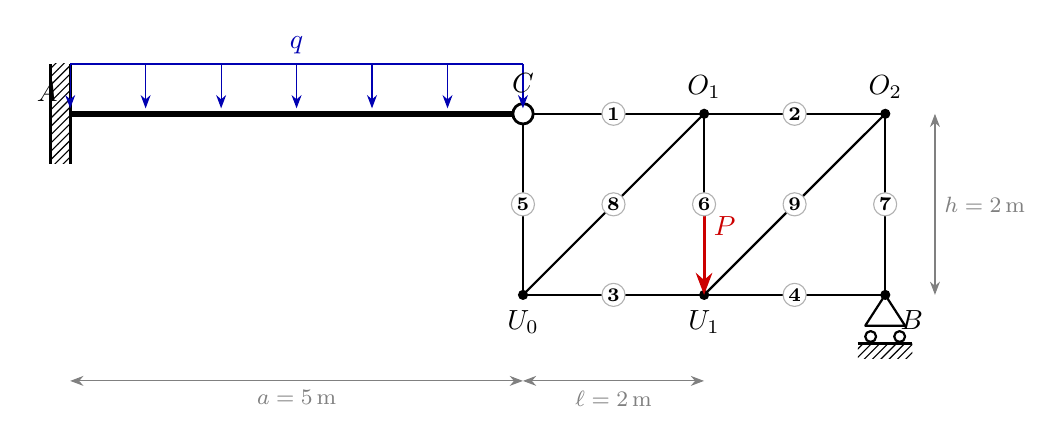
\begin{tikzpicture}[scale=1.15, >=Stealth, line join=round]
  \coordinate (A) at (0.000,0.000);
  \coordinate (C) at (5.000,0.000);
  \coordinate (O1) at (7.000,0.000);
  \coordinate (O2) at (9.000,0.000);
  \coordinate (U0) at (5.000,-2.000);
  \coordinate (U1) at (7.000,-2.000);
  \coordinate (U2) at (9.000,-2.000);
  \draw[thick] (C) -- (O1);
  \draw[thick] (O1) -- (O2);
  \draw[thick] (U0) -- (U1);
  \draw[thick] (U1) -- (U2);
  \draw[thick] (C) -- (U0);
  \draw[thick] (O1) -- (U1);
  \draw[thick] (O2) -- (U2);
  \draw[thick] (U0) -- (O1);
  \draw[thick] (U1) -- (O2);
  \draw[line width=2.2pt] (A) -- (C);
  \fill (C) circle (1.6pt);
  \fill (O1) circle (1.6pt);
  \fill (O2) circle (1.6pt);
  \fill (U0) circle (1.6pt);
  \fill (U1) circle (1.6pt);
  \fill (U2) circle (1.6pt);
  \draw[fill=white,line width=1pt] (C) circle (3.2pt);
  \draw[line width=1.1pt] (0.000,-0.550) -- (0.000,0.550);
  \fill[pattern=north east lines] (-0.220,-0.550) rectangle (0.000,0.550);
  \draw[line width=1.1pt] (-0.220,-0.550) -- (-0.220,0.550);
  \draw[thick] (9.000,-2.000) -- (8.780,-2.340) -- (9.220,-2.340) -- cycle;
  \draw[thick] (8.840,-2.460) circle (0.06) (9.160,-2.460) circle (0.06);
  \draw[line width=1.1pt] (8.700,-2.540) -- (9.300,-2.540);
  \fill[pattern=north east lines] (8.700,-2.700) rectangle (9.300,-2.540);
  \draw[blue!70!black,thick] (0.000,0.550) -- (5.000,0.550);
  \draw[->,blue!70!black] (0.000,0.550) -- (0.000,0.06);
  \draw[->,blue!70!black] (0.833,0.550) -- (0.833,0.06);
  \draw[->,blue!70!black] (1.667,0.550) -- (1.667,0.06);
  \draw[->,blue!70!black] (2.500,0.550) -- (2.500,0.06);
  \draw[->,blue!70!black] (3.333,0.550) -- (3.333,0.06);
  \draw[->,blue!70!black] (4.167,0.550) -- (4.167,0.06);
  \draw[->,blue!70!black] (5.000,0.550) -- (5.000,0.06);
  \node[blue!70!black,above] at (2.500,0.550) {$q$};
  \draw[->,red!80!black,line width=1.1pt] (7.000,-1.050) -- (7.000,-2.000);
  \node[red!80!black,above right] at (7.000,-1.450) {$P$};
  \node[circle,fill=white,draw=gray!60,inner sep=0.7pt,font=\scriptsize] at (6.000,0.000) {\textbf{1}};
  \node[circle,fill=white,draw=gray!60,inner sep=0.7pt,font=\scriptsize] at (8.000,0.000) {\textbf{2}};
  \node[circle,fill=white,draw=gray!60,inner sep=0.7pt,font=\scriptsize] at (6.000,-2.000) {\textbf{3}};
  \node[circle,fill=white,draw=gray!60,inner sep=0.7pt,font=\scriptsize] at (8.000,-2.000) {\textbf{4}};
  \node[circle,fill=white,draw=gray!60,inner sep=0.7pt,font=\scriptsize] at (5.000,-1.000) {\textbf{5}};
  \node[circle,fill=white,draw=gray!60,inner sep=0.7pt,font=\scriptsize] at (7.000,-1.000) {\textbf{6}};
  \node[circle,fill=white,draw=gray!60,inner sep=0.7pt,font=\scriptsize] at (9.000,-1.000) {\textbf{7}};
  \node[circle,fill=white,draw=gray!60,inner sep=0.7pt,font=\scriptsize] at (6.000,-1.000) {\textbf{8}};
  \node[circle,fill=white,draw=gray!60,inner sep=0.7pt,font=\scriptsize] at (8.000,-1.000) {\textbf{9}};
  \node[above left=1pt] at (A) {$A$};
  \node[above=4pt] at (C) {$C$};
  \node[above=2pt] at (O1) {$O_{1}$};
  \node[above=2pt] at (O2) {$O_{2}$};
  \node[below=2pt] at (U0) {$U_{0}$};
  \node[below=2pt] at (U1) {$U_{1}$};
  \node[below right=2pt] at (U2) {$B$};
  \draw[<->,gray] (0.000,-2.950) -- (5.000,-2.950) node[midway,below,font=\footnotesize]{$a=5$\,m};
  \draw[<->,gray] (5.000,-2.950) -- (7.000,-2.950) node[midway,below,font=\footnotesize]{$\ell=2$\,m};
  \draw[<->,gray] (9.550,0) -- (9.550,-2.000) node[midway,right,font=\footnotesize]{$h=2$\,m};
\end{tikzpicture}
\end{center}
\par\medskip\textbf{1.\ Static determinacy}\\[-2pt]
Counting criterion $n = r - (3 + v)$ with $r$ support reactions and $v$ hinge conditions:
\[ n = r - (3+v) = 4 - (3+1) = 0 \quad\Rightarrow\quad \text{the system is statically determinate.} \]
\par\medskip\textbf{2.\ Support reactions and hinge force}\\[-2pt]
$A_x = 0$\,kN,\quad $A_y = 32.5$\,kN,\quad $M_A = 100$\,kNm,\quad $B_y = 7.5$\,kN\\[2pt]$C_x = 0$\,kN,\quad $C_y = -7.5$\,kN\par
\par\medskip\textbf{3.\ Truss member forces}\par
\begin{center}\renewcommand{\arraystretch}{1.15}
\begin{tabular}{c r l}
\toprule
Member & Member force $S$ [kN] & Type \\
\midrule
  1 (C\,--\,O1) & 0 & zero-force \\
  2 (O1\,--\,O2) & -7.5 & compression \\
  3 (U0\,--\,U1) & 7.5 & tension \\
  4 (U1\,--\,U2) & 0 & zero-force \\
  5 (C\,--\,U0) & 7.5 & tension \\
  6 (O1\,--\,U1) & 7.5 & tension \\
  7 (O2\,--\,U2) & -7.5 & compression \\
  8 (U0\,--\,O1) & -10.61 & compression \\
  9 (U1\,--\,O2) & 10.61 & tension \\
\bottomrule
\end{tabular}\end{center}
\begin{center}
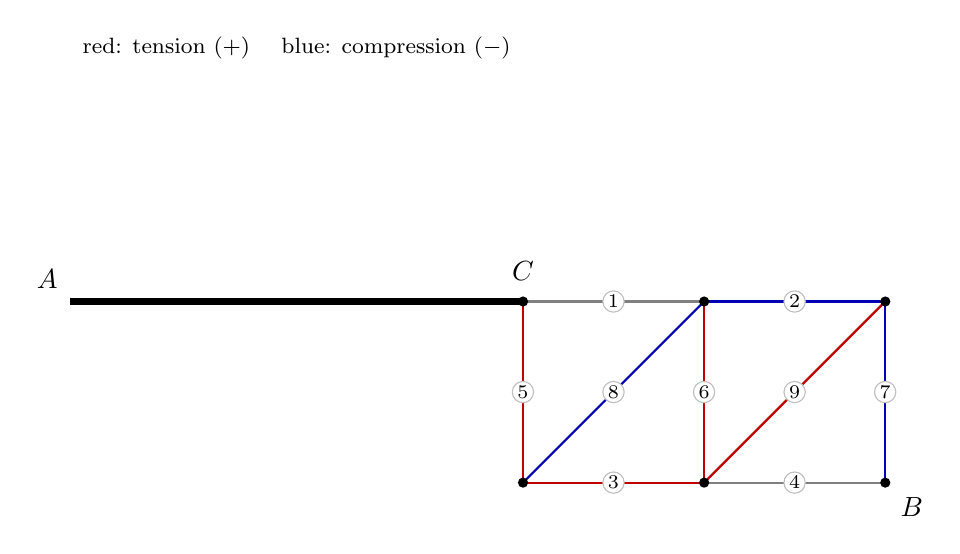
\begin{tikzpicture}[scale=1.15, >=Stealth, line join=round]
  \coordinate (A) at (0.000,0.000);
  \coordinate (C) at (5.000,0.000);
  \coordinate (O1) at (7.000,0.000);
  \coordinate (O2) at (9.000,0.000);
  \coordinate (U0) at (5.000,-2.000);
  \coordinate (U1) at (7.000,-2.000);
  \coordinate (U2) at (9.000,-2.000);
  \draw[thick,gray] (C) -- (O1);
  \draw[thick,blue!70!black] (O1) -- (O2);
  \draw[thick,red!75!black] (U0) -- (U1);
  \draw[thick,gray] (U1) -- (U2);
  \draw[thick,red!75!black] (C) -- (U0);
  \draw[thick,red!75!black] (O1) -- (U1);
  \draw[thick,blue!70!black] (O2) -- (U2);
  \draw[thick,blue!70!black] (U0) -- (O1);
  \draw[thick,red!75!black] (U1) -- (O2);
  \draw[line width=2.2pt] (A) -- (C);
  \fill (C) circle (1.6pt);
  \fill (O1) circle (1.6pt);
  \fill (O2) circle (1.6pt);
  \fill (U0) circle (1.6pt);
  \fill (U1) circle (1.6pt);
  \fill (U2) circle (1.6pt);
  \node[circle,fill=white,draw=gray!50,inner sep=0.6pt,font=\scriptsize] at (6.000,0.000) {1};
  \node[circle,fill=white,draw=gray!50,inner sep=0.6pt,font=\scriptsize] at (8.000,0.000) {2};
  \node[circle,fill=white,draw=gray!50,inner sep=0.6pt,font=\scriptsize] at (6.000,-2.000) {3};
  \node[circle,fill=white,draw=gray!50,inner sep=0.6pt,font=\scriptsize] at (8.000,-2.000) {4};
  \node[circle,fill=white,draw=gray!50,inner sep=0.6pt,font=\scriptsize] at (5.000,-1.000) {5};
  \node[circle,fill=white,draw=gray!50,inner sep=0.6pt,font=\scriptsize] at (7.000,-1.000) {6};
  \node[circle,fill=white,draw=gray!50,inner sep=0.6pt,font=\scriptsize] at (9.000,-1.000) {7};
  \node[circle,fill=white,draw=gray!50,inner sep=0.6pt,font=\scriptsize] at (6.000,-1.000) {8};
  \node[circle,fill=white,draw=gray!50,inner sep=0.6pt,font=\scriptsize] at (8.000,-1.000) {9};
  \node[above left=1pt] at (A) {$A$};
  \node[above=4pt] at (C) {$C$};
  \node[below right=2pt] at (U2) {$B$};
  \node[font=\footnotesize,align=center] at (2.50,2.80) {red: tension $(+)$ \quad blue: compression $(-)$};
\end{tikzpicture}
\end{center}
\par\medskip\textbf{4.\ Section-force diagrams of the bending beam $A$--$C$}\par
\begin{center}
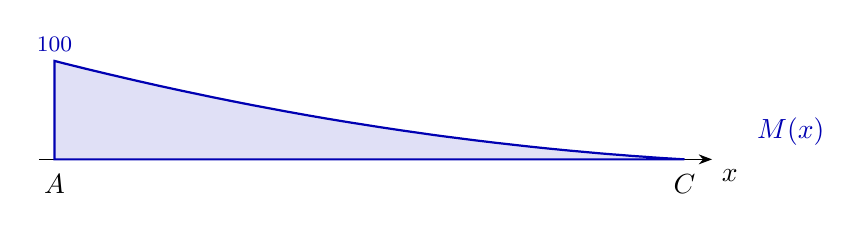
\begin{tikzpicture}[>=Stealth]
  \draw[->] (-0.2,0) -- (8.35,0) node[below right]{$x$};
  \node[below=2pt] at (0,0) {$A$};
  \node[below=2pt] at (8.00,0) {$C$};
  \filldraw[fill=blue!70!black!12,draw=blue!70!black,thick] (0,0) -- plot coordinates {(0.000,1.250) (0.133,1.216) (0.267,1.183) (0.400,1.150) (0.533,1.118) (0.667,1.086) (0.800,1.055) (0.933,1.024) (1.067,0.993) (1.200,0.963) (1.333,0.933) (1.467,0.904) (1.600,0.875) (1.733,0.847) (1.867,0.819) (2.000,0.791) (2.133,0.764) (2.267,0.737) (2.400,0.711) (2.533,0.685) (2.667,0.660) (2.800,0.635) (2.933,0.610) (3.067,0.586) (3.200,0.562) (3.333,0.539) (3.467,0.516) (3.600,0.494) (3.733,0.472) (3.867,0.451) (4.000,0.430) (4.133,0.409) (4.267,0.389) (4.400,0.369) (4.533,0.350) (4.667,0.331) (4.800,0.312) (4.933,0.294) (5.067,0.277) (5.200,0.260) (5.333,0.243) (5.467,0.227) (5.600,0.211) (5.733,0.196) (5.867,0.181) (6.000,0.166) (6.133,0.152) (6.267,0.138) (6.400,0.125) (6.533,0.112) (6.667,0.100) (6.800,0.088) (6.933,0.076) (7.067,0.065) (7.200,0.055) (7.333,0.044) (7.467,0.035) (7.600,0.025) (7.733,0.016) (7.867,0.008) (8.000,-0.000)} -- (8.000,0) -- cycle;
  \node[above,blue!70!black,font=\footnotesize] at (0.000,1.250) {100};
  \node[blue!70!black,right] at (8.80,0.35) {$M(x)$};
\end{tikzpicture}
\\[6pt]
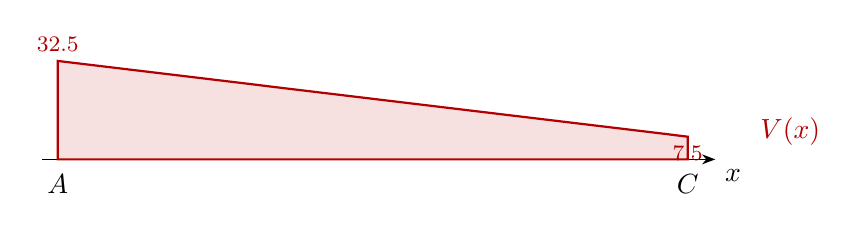
\begin{tikzpicture}[>=Stealth]
  \draw[->] (-0.2,0) -- (8.35,0) node[below right]{$x$};
  \node[below=2pt] at (0,0) {$A$};
  \node[below=2pt] at (8.00,0) {$C$};
  \filldraw[fill=red!70!black!12,draw=red!70!black,thick] (0,0) -- plot coordinates {(0.000,1.250) (0.133,1.234) (0.267,1.218) (0.400,1.202) (0.533,1.186) (0.667,1.170) (0.800,1.154) (0.933,1.138) (1.067,1.122) (1.200,1.106) (1.333,1.090) (1.467,1.074) (1.600,1.058) (1.733,1.042) (1.867,1.026) (2.000,1.010) (2.133,0.994) (2.267,0.978) (2.400,0.962) (2.533,0.946) (2.667,0.929) (2.800,0.913) (2.933,0.897) (3.067,0.881) (3.200,0.865) (3.333,0.849) (3.467,0.833) (3.600,0.817) (3.733,0.801) (3.867,0.785) (4.000,0.769) (4.133,0.753) (4.267,0.737) (4.400,0.721) (4.533,0.705) (4.667,0.689) (4.800,0.673) (4.933,0.657) (5.067,0.641) (5.200,0.625) (5.333,0.609) (5.467,0.593) (5.600,0.577) (5.733,0.561) (5.867,0.545) (6.000,0.529) (6.133,0.513) (6.267,0.497) (6.400,0.481) (6.533,0.465) (6.667,0.449) (6.800,0.433) (6.933,0.417) (7.067,0.401) (7.200,0.385) (7.333,0.369) (7.467,0.353) (7.600,0.337) (7.733,0.321) (7.867,0.304) (8.000,0.288)} -- (8.000,0) -- cycle;
  \node[above,red!70!black,font=\footnotesize] at (0.000,1.250) {32.5};
  \node[below,red!70!black,font=\footnotesize] at (8.000,0.288) {7.5};
  \node[red!70!black,right] at (8.80,0.35) {$V(x)$};
\end{tikzpicture}
\\[6pt]
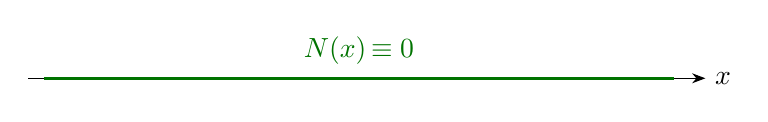
\begin{tikzpicture}[>=Stealth]
  \draw[->] (-0.2,0) -- (8.40,0) node[right]{$x$};
  \draw[green!45!black,very thick] (0,0) -- (8,0);
  \node[green!45!black] at (4,0.35) {$N(x)$\,$\equiv 0$};
\end{tikzpicture}
\end{center}
\end{document}